\section{Network Hardware and Architecture}
\label{evaluation-sec-architecture}

\subsection{Hardware}

\begin{figure}[t]
\begin{center}
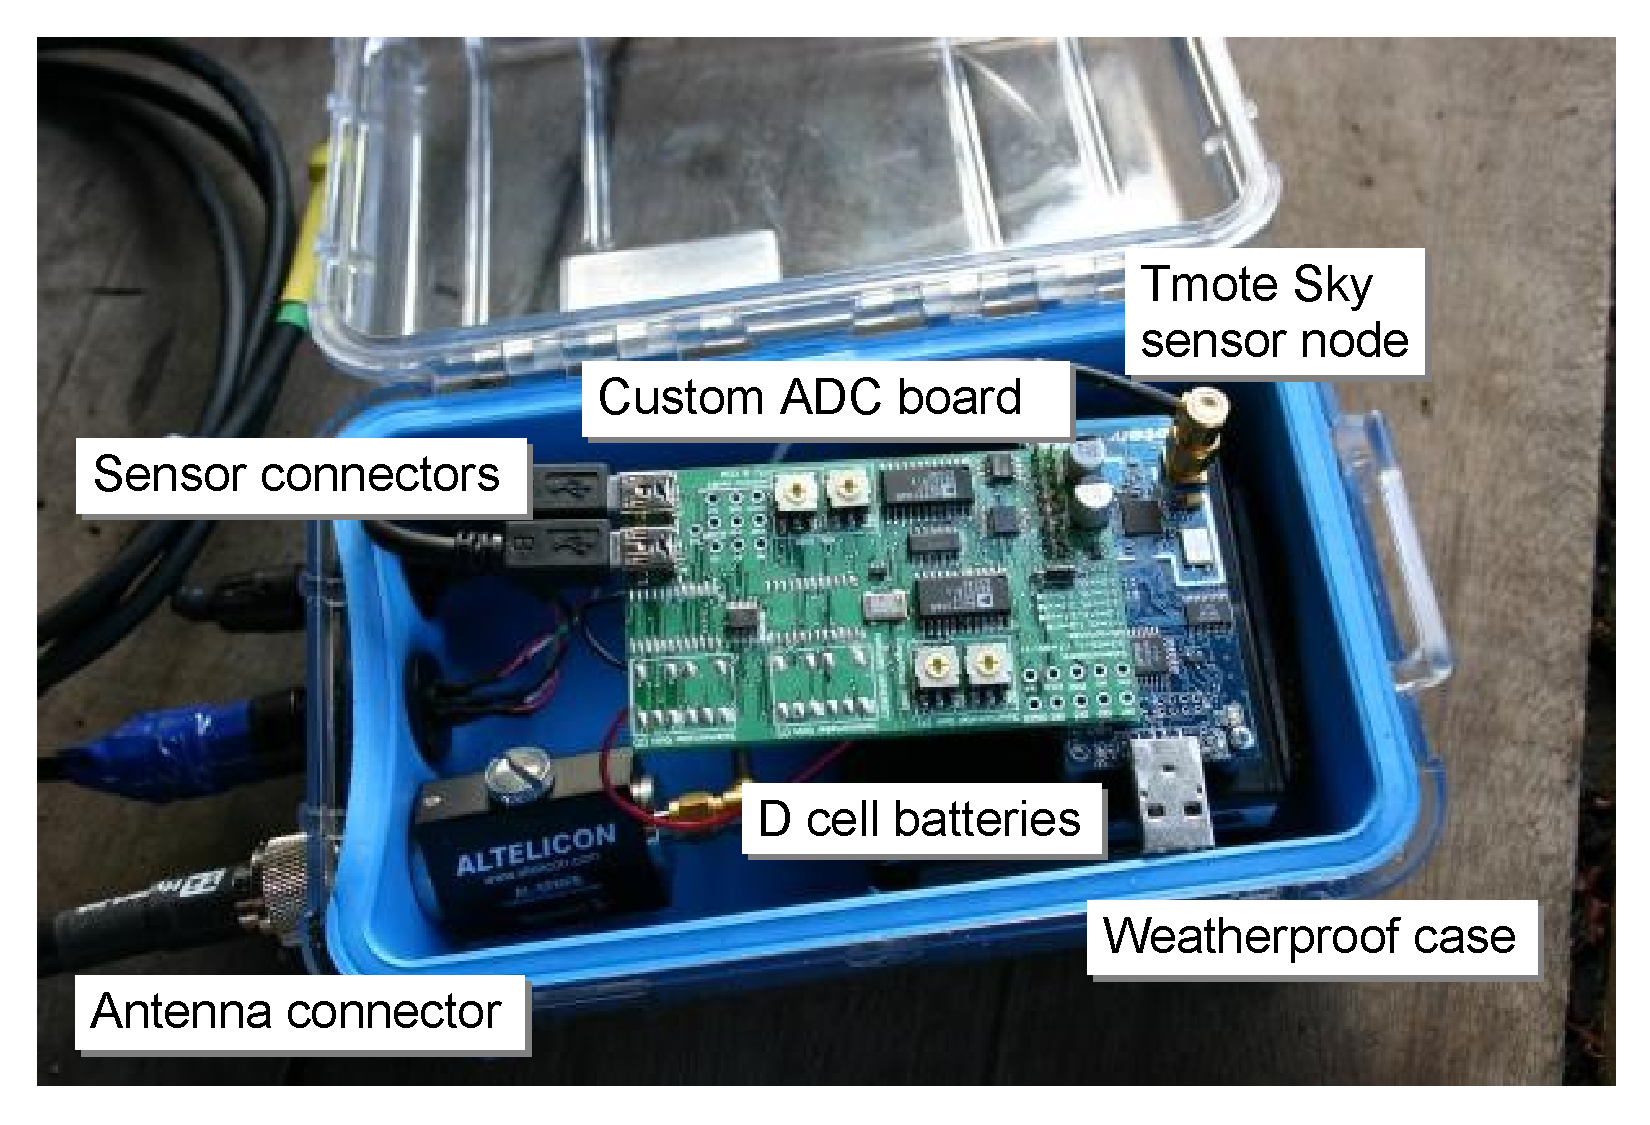
\includegraphics[width=1.0\hsize]{./3-evaluation/figs/node.pdf}
\end{center}
\caption{\textbf{Our wireless volcano monitoring sensor node.}}
\label{evaluation-fig-node}
\end{figure}

Our volcano monitoring sensor station consists of a Moteiv TMote
Sky~\cite{moteiv} wireless sensor network node, an 8~dBi~2.4GHz external
omnidirectional antenna, one or more seismometers, a microphone, and a custom
hardware interface board. An example node with components labeled is shown in
Figure~\ref{evaluation-fig-node}.

The TMote Sky is a descendant of the UC Berkeley Mica ``mote'' sensor node.
It features a Texas Instruments MSP430 microcontroller, 48~kB of program
memory, 10~kB of SRAM, 1~MB of external flash memory and a 2.4GHz Chipcon
CC2420 IEEE 802.11.4 radio. The TMote Sky was designed to run
TinyOS~\cite{tinyos-asplos00}, and all of our software development made use
of this environment. We chose the TMote Sky for several reasons. The MSP430
microprocessor provides a large number of configurable ports, easily
supporting external devices, and the large amount of flash memory was useful
for buffering collected data.

We built a custom hardware board to integrate the TMote Sky with the
seismoacoustic sensors. The board features up to four Texas Instruments
AD7710 analog to digital converters (ADCs) providing up to 24~bits per
channel of resolution. Although the MSP430 microcontroller provides on-board
ADCs, they are unsuitable for our application. First, they provide only
16~bits of resolution while we required at least 20~bits. Second,
seismoacoustic signals require an aggressive filter centered around 50~Hz.
Due to the infeasibility of implementing such a filter using analog
components, it is usually approximated digitally, requiring several factors
of oversampling. To perform this filtering, the AD7710 is sampling at over
30~kHz while presenting an output word rate of 100~Hz. The high sample rate
and computation required by digital filtering are best delegated to a
specialized device.

Each sensor node was powered by a pair of alkaline D~cell batteries.
Anticipating a remote network location, D~cells provided the best combination
of low cost, high capacity, and ready availability, and are able to power a
node for over a week. Approximately 75\% of the power drawn by each node is
consumed by the sensor interface board, primarily due to the high power
consumption of the ADCs. 

For sensors, nodes are fitted with either a Geospace Industrial GS-11
geophone --- a single-axis seismometer with a corner frequency of 4.5~Hz,
oriented in the vertical plane of motion --- or triaxial Geospace Industries
GS-1 seismometers with corner frequencies of 1~Hz, yielding separate signals
in each of the three axes. Both sensors are passive instruments: ground
motion generates a voltage which is amplified and digitized by the sampling
board. In addition, each node was attached to an omnidirectional microphone,
the Panasonic WM-034BY. This microphone has been used in other infrasonic
monitoring studies~\cite{johnson-etal-04b}.

\subsection{Network Operation}

Given the current capabilities of wireless sensor network nodes, we set out
to design a data collection network meeting the application's scientific
requirements Before motivating and explaining our design we provide a
high-level overview of typical network operation.
Figure~\ref{evaluation-fig-architecture} outlines the main system components.

\begin{figure}[t]
\begin{center}
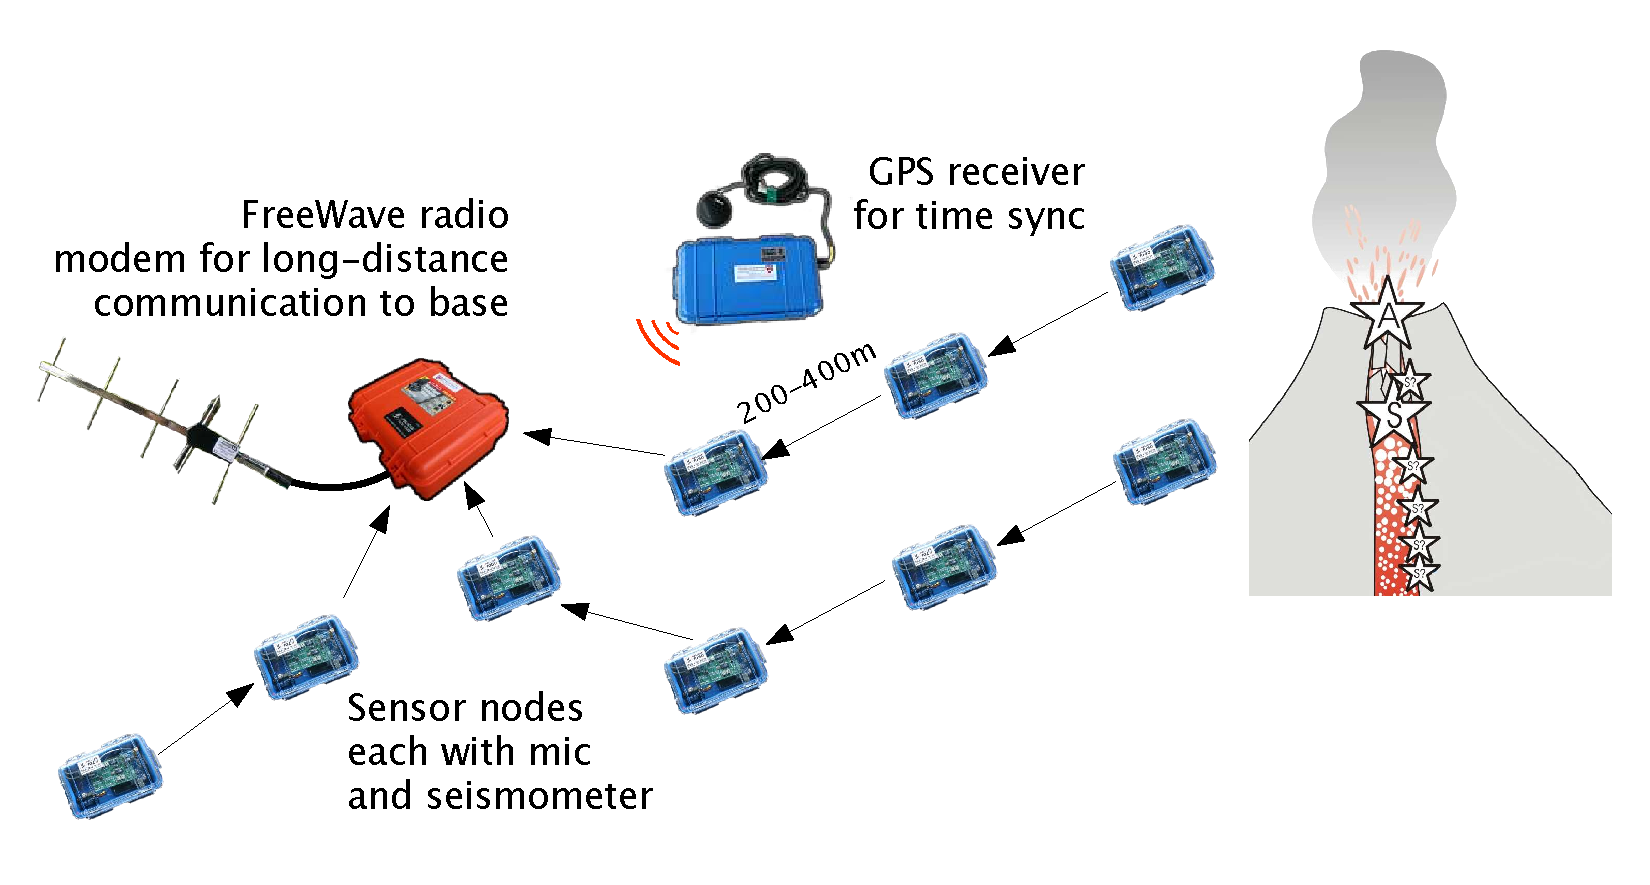
\includegraphics[width=0.7\hsize]{./3-evaluation/figs/architecture.pdf}
\end{center}
\caption{\textbf{Schematic representation of our sensor network
architecture.}}
\label{evaluation-fig-architecture}
\end{figure}

Each node samples two or four channels of seismoacoustic data at 100~Hz,
storing the data in local flash memory. Nodes also transmit periodic status
messages and participate in routing and time-synchronization protocols. When
a node detects an interesting event, it routes a message to the base station
laptop. If enough nodes report an event within a short time interval, the
laptop initiates data collection which proceeds in a round-robin fashion.
Between 30~and~60~s of data is downloaded from each node with a reliable data
collection protocol, ensuring that all buffered data from the event is
retrieved. When data collection completes, nodes return to sampling and
storing sensor data.

\subsection{Overcoming High Data Rates: Event Detection and Buffering}

When designing high data-rate sensing applications an important limitation of
current sensor network nodes is low radio bandwidth. IEEE 802.15.4 radios,
such as the Chipcon CC2420, have raw data rates of around 30~kBps. However
overheads caused by packet framing, medium access control (MAC), and multihop
routing reduce the achievable data rate to less than 10~kBps even in a
single-hop network. Because of the high data rates involved (600-1200~Bps
from each node) it is infeasible to continuously transmit all sensor data.

Rather, nodes are programmed to locally detect interesting seismic events and
transmit event reports to the base station. If enough nodes trigger in a
short time interval, the base station attempts to download the last 60~s of
data from each node. This design forgoes continuous data collection for
increased resolution following significant seismic events, which include
earthquakes, eruptions, or long-period (LP) events, such as tremor. The
download window of 60~s was chosen to capture the bulk of the eruptive and
earthquake events, although many LP events can exceed this window (sometimes
lasting minutes or hours). To validate our network against existing
scientific instrumentation, our network was designed for high-resolution
signal collection rather than extensive in-network processing.

Sampled data is stored in the local flash memory of the node, which is
treated as a circular buffer. Each block of data is timestamped using the
local node time, which can later be mapped onto a global time, as explained
in Section~\ref{evaluation-subsec-timerectification}. Each node runs an
\textit{event detector} on locally-sampled data. Good event detection
algorithms produce high event-detection rates while maintaining small
false-positive rates. The sensitivity of the detection algorithm links these
two metrics: a more sensitive detector correctly identifies more events at
the expense of producing more false positives. We evaluate the performance of
our event detection algorithm further in
Section~\ref{evaluation-sec-eventdetection}.

The data set produced by our previous deployment at Tungurahua
volcano~\cite{volcano-ewsn05} aided in the design of the event detector. We
implemented a short-term average/long-term average threshold detector, which
computes two exponentially-weighted moving averages (EWMAs) with different
gain constants. When the ratio between short-term average and the long-term
average exceeds a fixed threshold, the detector fires. The detector threshold
allows nodes to distinguish between low-amplitude signals, perhaps caused by
distant earthquakes, and high-amplitude signals caused by nearby volcanic
activity.

When the event detector on a node fires it routes a small message to the base
station laptop. If the base station receives triggers from 30\% of the active
nodes within a given time window, the laptop initiates data collection from
the entire network, including nodes that did not report the event. This
global filtering prevents spurious event detections from triggering a data
collection cycle. Because nodes can only buffer 20 minutes of eruption data
locally each, and data collection from the entire network may exceed this
envelope (we found that fetching 60~s of data from 16 nodes takes over 1
hour) each node pauses sampling and reporting events until its data has been
uploaded.

\subsection{Reliable Data Transmission and Time Synchronization}

Extracting high-fidelity data from a wireless sensor network is challenging
for two primary reasons. First, radio links are lossy and frequently
asymmetrical. Second, low-cost crystal oscillators on sensor nodes have low
tolerances and so clock rates vary across the network. Much prior research
has focused on addressing these challenges.

We developed a reliable data-collection protocol, called \texttt{Fetch}, that
retrieves buffered data from each node over a multihop network. Samples are
buffered locally in \textit{blocks} of 256~B, tagged with a sequence number
and timestamp. During transmission each requested block is fragmented into a
number of \textit{chunks}, each sent in a single radio message. The base
station laptop retrieves a block by flooding a request to the network using
\texttt{Drip}, a variant of the TinyOS \texttt{Trickle}~\cite{trickle}
data-dissemination protocol. The request contains the target node ID, the
block sequence number, and a bitmap identifying missing chunks in the block. 

The target node replies by sending the requested chunks over a multihop path
to the base station. The routing tree is constructed using
\texttt{MultiHopLQI}, a variant of the TinyOS
\texttt{MintRoute}~\cite{awoo-multihop} routing protocol modified to select
routes based on the CC2420 Link Quality Indicator (LQI) metric. Link-layer
acknowledgments and retransmissions are used at each hop to improve
reliability. Retrieving one minute of stored data from a two-channel sensor
node requires fetching 206~blocks and can takes several minutes to complete,
depending on the quality of the multihop path and the node's depth in the
routing tree. We evaluate the performance of Fetch in more detail in
Section~\ref{evaluation-sec-performance}.

Scientific volcano studies require that sampled data be accurately
timestamped. In our case, a global clock accuracy of 1~ms was sufficient. We
chose to use the Flooding Time Synchronization Protocol (FTSP)~\cite{ftsp} to
establish a global clock across our network. The published accuracy of FTSP
is very high and the TinyOS code was straightforward to integrate into our
application. One of the nodes used a Garmin GPS receiver to map the FTSP
global time to GMT. Unfortunately, FTSP protocol failures during our field
deployment made assigning accurate timestamps quite challenging, as
documentented in Section~\ref{evaluation-sec-timing}.

\subsection{Command and Control}

A feature missing from most traditional volcanic data acquisition equipment
is real-time network control and monitoring. The long-distance radio link
between the observatory and the sensor network allowed the laptop to monitor
and control the network's activity. Every 10~s, each node transmits a
\textit{status message} to the base station that includes its position in the
routing tree, buffer status, local and global timestamps, battery voltage,
and other information. In addition, the base station can issue a
\textit{command} to each node, instructing it to respond with an immediate
status message, start or stop data sampling, and set various software
parameters. 

We developed a Java-based GUI for monitoring the network's behavior and
manually setting parameters, such as sampling rates and event detection
thresholds. In addition, the GUI was responsible for controlling data
collection following a triggered event, moving significant complexity out of
the sensor network. All packets received by the laptop from the sensor
network were logged, facilitating later analysis of the network's operation.

The GUI also displayed a table summarizing network state, based on the
periodic status messages transmitted by each node. Each table entry included
the node ID; local and global timestamps; various status flags; the amount of
locally-stored data; depth, parent, and radio link quality in the routing
tree; and the node's temperature and battery voltage. This functionality
greatly aided sensor deployment, as a team member could rapidly determine
whether a new node had joined the network and the quality of its radio
connectivity.
